\chapter{Cross-platform development}
\label{S:cp-develompent}

In the early begining of computers, each manufacturer had to decide how to access to
their hardware functionalities. Since there were no standards for some cases,
the first inter-compatibility problems started to appear because programs were
not able to run on different computers.

When Operative Systems (OS) appeared, they started to use drivers. A driver is
an interface that maps logic functions (for instance, turn on a led) to hardware
operations (short circuit some part of the electronics). Those drivers are
often provided by manufacturers to let its hardware work when using an OS.

Nowadays desktop applications are not programmed directly for a specific 
hardware. OS are in charge to expose an application programming interface (API)
to access those functionalities.

For a software, being cross-platform means being able to run on different OS. However, since the APIs
exposed by the OSs are not equal, programs are not cross-platform by default.

\section{Technological soup}

Lots of technologies has been created aimed to writing just one code that runs
in as many platforms as possible. The motivation to achieve this goal is
obvious, to reduce the development cost. But, as opposed to this gain, it
results in some performance reduction.

Most intuitive solution is to use cross-platform frameworks. Those have
conditionals that uses an API function or another depending on which operative
system is used to compile the library.

But the common way is with scripting programming languages. Those are human
readable strings that are interpreted by a program called interpreter during
execution time. One step further is to compile the source code into an
intermediate pseudo-machine code that is easier to understand for the
interpreter. This second group is known as virtual machine programming
languages. Their main advantage is that programs run faster, but in contrast,
developers lose some time compiling the code each time they want to test the
application. Both technologies can run over all the platforms that its
interpreter supports.

The last solution is to use transcompilers or source-to-source compilers.
They translate from one programming language to many others. This translation
could be done into a scripting language (there intercompatiblity is provided) or
can make a specific translation to a compiled language depending on the OS.

\begin{figure}[htb]
	\begin{center}
		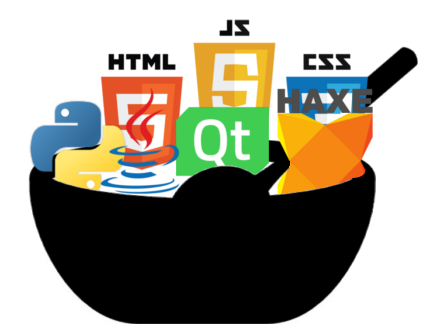
\includegraphics[width=0.5\textwidth]{./figures/techsoup.png}
		\caption{Some cross-platform technologies}
		\label{F:tech-soup}
	\end{center}
\end{figure}


More than twenty years putting effort to solve this problem has created a 
technological soup (Figure \ref{F:tech-soup}). Qt, Python, JavaScript, Java and 
Haxe
\cite{qt-web}\cite{py-web}\cite{js-wiki}\cite{what-is-java}\cite{what-is-haxe}
are some examples among many others.

\subsection{Qt}

Qt is a complete cross-platform software framework with ready-made UI elements,
\CC libraries, and a complete integrated development environment with tools for 
everything you need to develop software for any project \cite{qt-web}.

\begin{codefigure}
	\cppexternal[
		caption=Qt hello world,
		label=L:qt-hello-world,
		%
		classoffset=1,
		morekeywords={QPushButton, QApplication}
	]{source/qt_hello_world.cpp}
\end{codefigure}

Code of Listing \ref{L:qt-hello-world} creates a window and add a button that
says Hello World with size 100x30.

\subsection{Python}

Python is an example of a scripting programming language. The main design rule
was to be very easy to read. For this reason, Python is the only language where
tabulation rules must be strictly followed to make the program work.

It is also considered an object-oriented language suitable for many purposes.
It has a clear, intuitive syntax, powerful high-level data structures, and a
flexible dynamic type system \cite{An93pythonfor}.

Python is often used to create terminal programs or web services because GUI
are not supported by default, but there are many frameworks that can be used,
for instance, \textbf{Kivy}.

\begin{codefigure}
	\pythonexternal[
		caption=Kivy hello world,
		label=L:kivy-hello-world,
	]{source/kivy_hello_world.py}
\end{codefigure}

As Listing \ref{L:kivy-hello-world} shows up, a window with is created with a
button which text is "Hello World".

\subsection{JavaScript}

JavaScript is also a well-know widely-used scripting programming language. It is commonly used
alongside with HTML and CSS as core technologies to make webpages. Moreover, due
to its flexibility, it is used in many other fields like game programming or
desktop applications.

It has many interpreters but all of them has to fulfill ECMAScript
specification. V8 is an example of JavaScript engine used in Google Chrome and
Node.js \cite{nodejs-web}. This latter example is widely used to build terminal
applications and web services.

Some years ago, developing trends were to create web applications instead of
desktop ones since it has less development cost and all platforms have browsers
indeed. For this reason, web technologies have grown a lot and today can be
compared with desktop technologies.

But web applications have several technological problems. The main one is that
since the code is download from an external non-trusted source, the browser
must limit the access to the computer for security reasons
\cite{securing-your-browser}. For instance, web applications can not read the
user's file system. Moreover, programs have higher load periods due to those
downloads.

Another important fact is that user experience (UX) will never be as good as
using a desktop application due to it is embedded inside the browser and some
space is lost due to menus.

% TODO: *** what about chrome/chromium apps, is it the same?***
% Respuesta: Realmente lo problematico es que el JavaScript del browser
% es mas limitado.

\subsubsection{Electron}

Electron is a Node.js framework that lets developers build cross-platform
desktop applications using JavaScript, HTML, and CSS \cite{electron-web}. As
seen before, web technologies are now able to race desktop ones in terms of
performance and scalability.

The idea behind Electron is take profit of the fact that Node.js and Chrome uses
the same JavaScript engine (V8) to let Node.js instantiate Chrome windows and
use them as user interface. Moreover, Electron Chrome windows are able to use
all extra Node.js modules, for instance, to be able to access the computer's
file system.

UX is improved respect web pages because Chrome menus are removed and
application code is now inside user's computer.

For short, Electron help developers to create cross-platform desktop 
applications using the same technologies that the ones used to create a webpage.

\subsubsection{NW.js}

NW.js, previously known as node-webkit, works on the contrary of Electron. It
is just a Chrome web browser where you can call all the node modules
\cite{nwjs-web}. So the main difference is the entry point of the application.
In Electron, the start point of your program execution is Node.js while on
NW.js the entry point is an HTML file.

\subsection{Java}

This well-known programming language is one of the most used to build
cross-platform desktop applications due to its maturity. Java is a
general-purpose, concurrent, class-based, object-oriented language and it is
designed to be easy to learn in order to let many programmers to have fluency
in the language \cite{java-8-specs}.

Classic compiled languages, such as, C and \CC, directly compile into machine
code, which is directly interpreted by the hardware. As opposed to C and \CC,
Java can be considered a virtual machine programming language.

\begin{codefigure}
	\javaexternal[
	caption=Java hello world,
	label=L:java-hello-world,
	%
	classoffset=1,
	morekeywords={HelloWorldApp}
	]{source/HelloWorldApp.java}
\end{codefigure}

Listing \ref{L:java-hello-world} is an example of Java program that prints the
test “Hello World!” into the terminal. All files must contain just one class and
the name of the file must match. The static function called main is the entry
point of the application and in this example uses the standard output to print
a message.

\subsection{Haxe}

Finally, Haxe is a high-level open source programming language that can be 
transcompiled many other languages. It has an ECMAScript-oriented syntax but 
with the peculiarity that can be typed \cite{what-is-haxe}. 

\begin{table}[htb]
\begin{center}
\begin{tabular}{|l|l|l|}
\hline
{\bf Name }		& {\bf Output Type} & {\bf Main usages}  \\ \hline \hline
JavaScript		& Sourcecode		& Browser, Desktop, Mobile, Server \\ \hline
Neko			& Bytecode			& Desktop, Server   \\ \hline
PHP				& Sourcecode		& Server   \\ \hline
Python			& Sourcecode		& Desktop, Server   \\ \hline
\CC				& Sourcecode		& Desktop, Mobile, Server   \\ \hline
ActionScript 3	& Sourcecode		& Browser, Desktop, Mobile   \\ \hline
Flash			& Bytecode			& Browser, Desktop, Mobile   \\ \hline
Java			& Sourcecode		& Desktop, Server   \\ \hline
C\#				& Sourcecode		& Desktop, Mobile, Server   \\ \hline
\end{tabular}
\caption{Haxe use cases \cite{what-is-haxe}}
\label{T:haxe-use-cases}
\end{center}
\end{table}

Table \ref{T:haxe-use-cases} shows up many languages in which Haxe can be
compiled. Then lets see a bit of Haxe syntax.

\begin{codefigure}
	\haxeexternal[
		caption=Haxe hello world,
		label=L:haxe-hello-world,
		%
		classoffset=1,
		morekeywords={Main}
	]{source/Main.hx}
\end{codefigure}

As we can see in Listing \ref{L:haxe-hello-world}, Haxe can be typed defining 
variables that way: \haxeinline{var text: String}. This code can be compiled
for example to Python other languages using the terminal command:

\begin{terminal}[caption=Haxe python transcompilation command, label=haxe-2-py]
%
\terminalcmd[haxe -main Main.hx -python main.py]
%
%\terminalcmd%

\end{terminal}

\section{Electron}
\label{S:electron}

The technology that fits better with the project's specifications is Electron. 
There are several projects like this one that are developed using this 
framework. Even it is probably not as mature as other ones, it had a big impact 
in the developers community. Figure \ref{F:electron-applications} shows several
applications developed using Electron \cite{electron-web}.

\begin{figure}[htb]
	\begin{center}
		\begin{subfigmatrix}{4}
			\subfigure[Visual Studio Code (Microsoft)]
			{
\includegraphics{./figures/vs-code-icon.png}\label{SF:S1}} 
			\subfigure[Atom]
			{
\includegraphics{./figures/atom-icon.png}\label{SF:S1}} 
			\subfigure[Github Desktop]
			{
\includegraphics{./figures/github-desktop-icon.png}\label{SF:S1}} 
			\subfigure[Slack]
			{
\includegraphics{./figures/slack-icon.png}\label{SF:S1}} 
		\end{subfigmatrix}
		\caption{Electron application examples}
		\label{F:electron-applications}
	\end{center}
\end{figure}

Moreover, the development of web applications has been evolved very fast with
the objective to have complex programs with a very good scalability and without
putting so much effort.

Then, some examples show how Electron works in a little more of detail.
Complete code is available on Appendix \ref{APP:electron-hello-world}.

\subsection{Main process}

% TODO: NO ENTIENDO EL COMOR?! jajaja
% JavaScript solo tiene un tread pero puedes tener muchos procesos en paralelo
% para hacer cosas a la vez. Osea:
%    - En C y Java puedes utilizar semaforos para acceder a memoria comparida.
%    - En javascript tienes que utilizar mecanismos de comunicacion como si
%      fueran aplicaciones diferentes.
% Otra cosa seria que desde un lenguaje multithreaded lances varios threads 
% corriendo javascript o que un modulo javascript hecho en C aplique 
% multithread.

JavaScript is a single threaded programming language. In order to be able to
work in parallel, Electron has several processes. The initial one is called 
main process. It is in charge of create all browser windows, communicate them,
to build application menus and control context events.

\begin{codefigure}
	\jsexternal[
		caption=Electron app events,
		label=L:electron-app-events
	]{source/electron-app.js}
\end{codefigure}

Code of Listing \ref{L:electron-app-events} is an example of the most common
handled events. The most important is the \textit{"ready"} event, where the
main window of the application is created.

\subsection{Browser window}

Once event \textit{"ready"} is called, browser windows can be created. Each
window has its own independent process called renderer. The way to create
windows is shown on Listing \ref{L:electron-create-window}.

\begin{codefigure}
	\jsexternal[
		caption=Electron window creation,
		label=L:electron-create-window,
	]{source/electron-create-window.js}
\end{codefigure}

Browser windows can be created using several parameters to define its initial
behavior, for instance: width, height, position, etc. They can load files  
using several protocols (HTTP, FTP, etc) or directly access to local hard disk.
In Electron, the most common way is to use local files to reduce load time and
let the application work without Internet connection. Finally, window objects
also have events, for example: \textit{"closed"}, \textit{"ready-to-show"},
\textit{"move"}\dots

\subsection{Interprocess communication}

Finally, to be able to communicate the main process and the renderer processes, 
Electron provides inter-process communication (IPC). By default, it can provide
communications main-to-renderer and renderer-to-main. Therefore, if
renderer-to-renderer communication is needed, a bridge must be implemented
inside the main process.

% TODO: Pongo ejemplo de codigo de esto tambien? 
% TODO: dependiendo del número final de páginas

\section{Web technologies}

Core World Wide Web technologies, as seen before, are JavaScript, HTML and CSS.
Nevertheless, there are many other specialized tools to solve specific deficits 
those technologies have. For instance, Typescript, SCSS and Gulp are used to
enhance scalability and maintainability. 

\subsection{Typescript}

Typescript\cite{typescript-web} is a programming language created by Microsoft
that is a typed superset of JavaScript that compiles to plain JavaScript. It has
two main advantages:

\begin{description}
	\item[Typed language]
	Since Typescript is a typed language and it has a compilation process, any
	mismatch of parameters used in a function call are detected before testing
	anything. Also, Integrated Development Environments (IDEs) can help
	developers highlight those mismatches because type information is provided.
	
	\item[Compiles to plain Javascript]
	There are many web browsers and not all of them support current ECMAScript 
	standard. Using TypeScript developers don't need to take care of it because
	target JavaScript version can be selected.

\end{description}

Many JavaScript libraries also provide its TypeScript typings. Using this 
information, the compiler can detect if the library is properly used.

\begin{codefigure}
	\tsexternal[
		caption=TypeScript example,
		label=L:typescript-example,
		%
		classoffset=1,
		morekeywords={Person, T, GreetingsCallback, Greetings}
	]{source/hello-world.ts}
\end{codefigure}

Listing \ref{L:typescript-example} is a TypeScript example that shows some
advanced type declarations. As can be seen, it supports templates, interfaces
and even defining function types.

Each time TypeScript is compiled, a tool called TsLint can be used to check if 
some programming style guides are followed. Follow this rules, even if it is 
not strongly needed, is very useful to keep code easy-to-read. For instance, 
a common rule used in JavaScript is to name variables following lower camel case
and upper camel case for classes.

\subsection{Sass}

Like TypeScript, SASS is a code transcompiler, but it translates from SASS to
CSS. It is designed to improve CSS functionalities.

\begin{codefigure}
	\sassexternal[
		caption=Sass example,
		label=L:sass-example,
		%
		classoffset=2,
		morekeywords={\$app_green, flex-row}
	]{source/example.scss}
\end{codefigure}

Listing \ref{L:sass-example} helps to see all the advantages that SASS provides.
The main ones are:

\begin{description}
	\item[Nesting CSS selectors]
	Improves code scalability. 

	\item[Variables]
	Helps to define palettes, sizes, etc.
	
	\item[Mixins]
	Similar to functions, they are very useful to define common behaviors.
	
\end{description}

\subsection{Gulp}

Gulp is a toolkit for automating painful or time-consuming tasks in your
development workflow, so you can stop messing around and build something
\cite{gulp-web}.

This project has several routine tasks, such as launch electron, compile
TypeScript and SASS each time a file change happens, etc. For this reason, 
several gulp tasks are created to help development.

\begin{codefigure}
	\jsexternal[
		caption=Gulp task to compile SASS,
		label=L:gulp-sass,
	]{source/gulp-sass.js}
\end{codefigure}

For instance, Listing \ref{L:gulp-sass} shows how a task to compile all .sass 
files is implemented.
